\section{Implementation details}\label{sec:impl}

In this chapter we will discuss the various tools and technologies that we ended up using to create our tool, including, but not limited to; choice of programming language, frameworks and libraries and discuss why we chose the ones we did.

Starting off with the programming language we went with, our choice was Kotlin. Kotlin is a new and exiting language on the JVM that has gotten a lot of attention in the recent years after Google announced they would make it an official language for Android development during their I/O conference back in 2017. While the language has since `branched out' with JavaScript transpilers and a native compiler, letting developers target different platforms, I would argue that one of the main strengths of the language is that despite being relatively young, it is able to tap into the vast number of libraries and tools written for the JVM by compiling down to Java-bytecode, allowing for full interoperability with Java. Among the other benefits of the language's relatively young age, is that it has been able to draw inspiration from other modern giving it features such as type inference, string interpolation and default values. This means that lends itself very well towards writing functional code despite being object oriented, through shorthands for lambda expressions, support for proper function types and distinctions between mutable and immutable structures and variables. As an added bonus, the language is also backed heavily by JetBrains, well known for their suite of IDEs and plugins such as IntelliJ, PyCharm and ReSharper, so the language also has first-class tooling support, making it easy to pick up. 

\begin{figure}[h]
	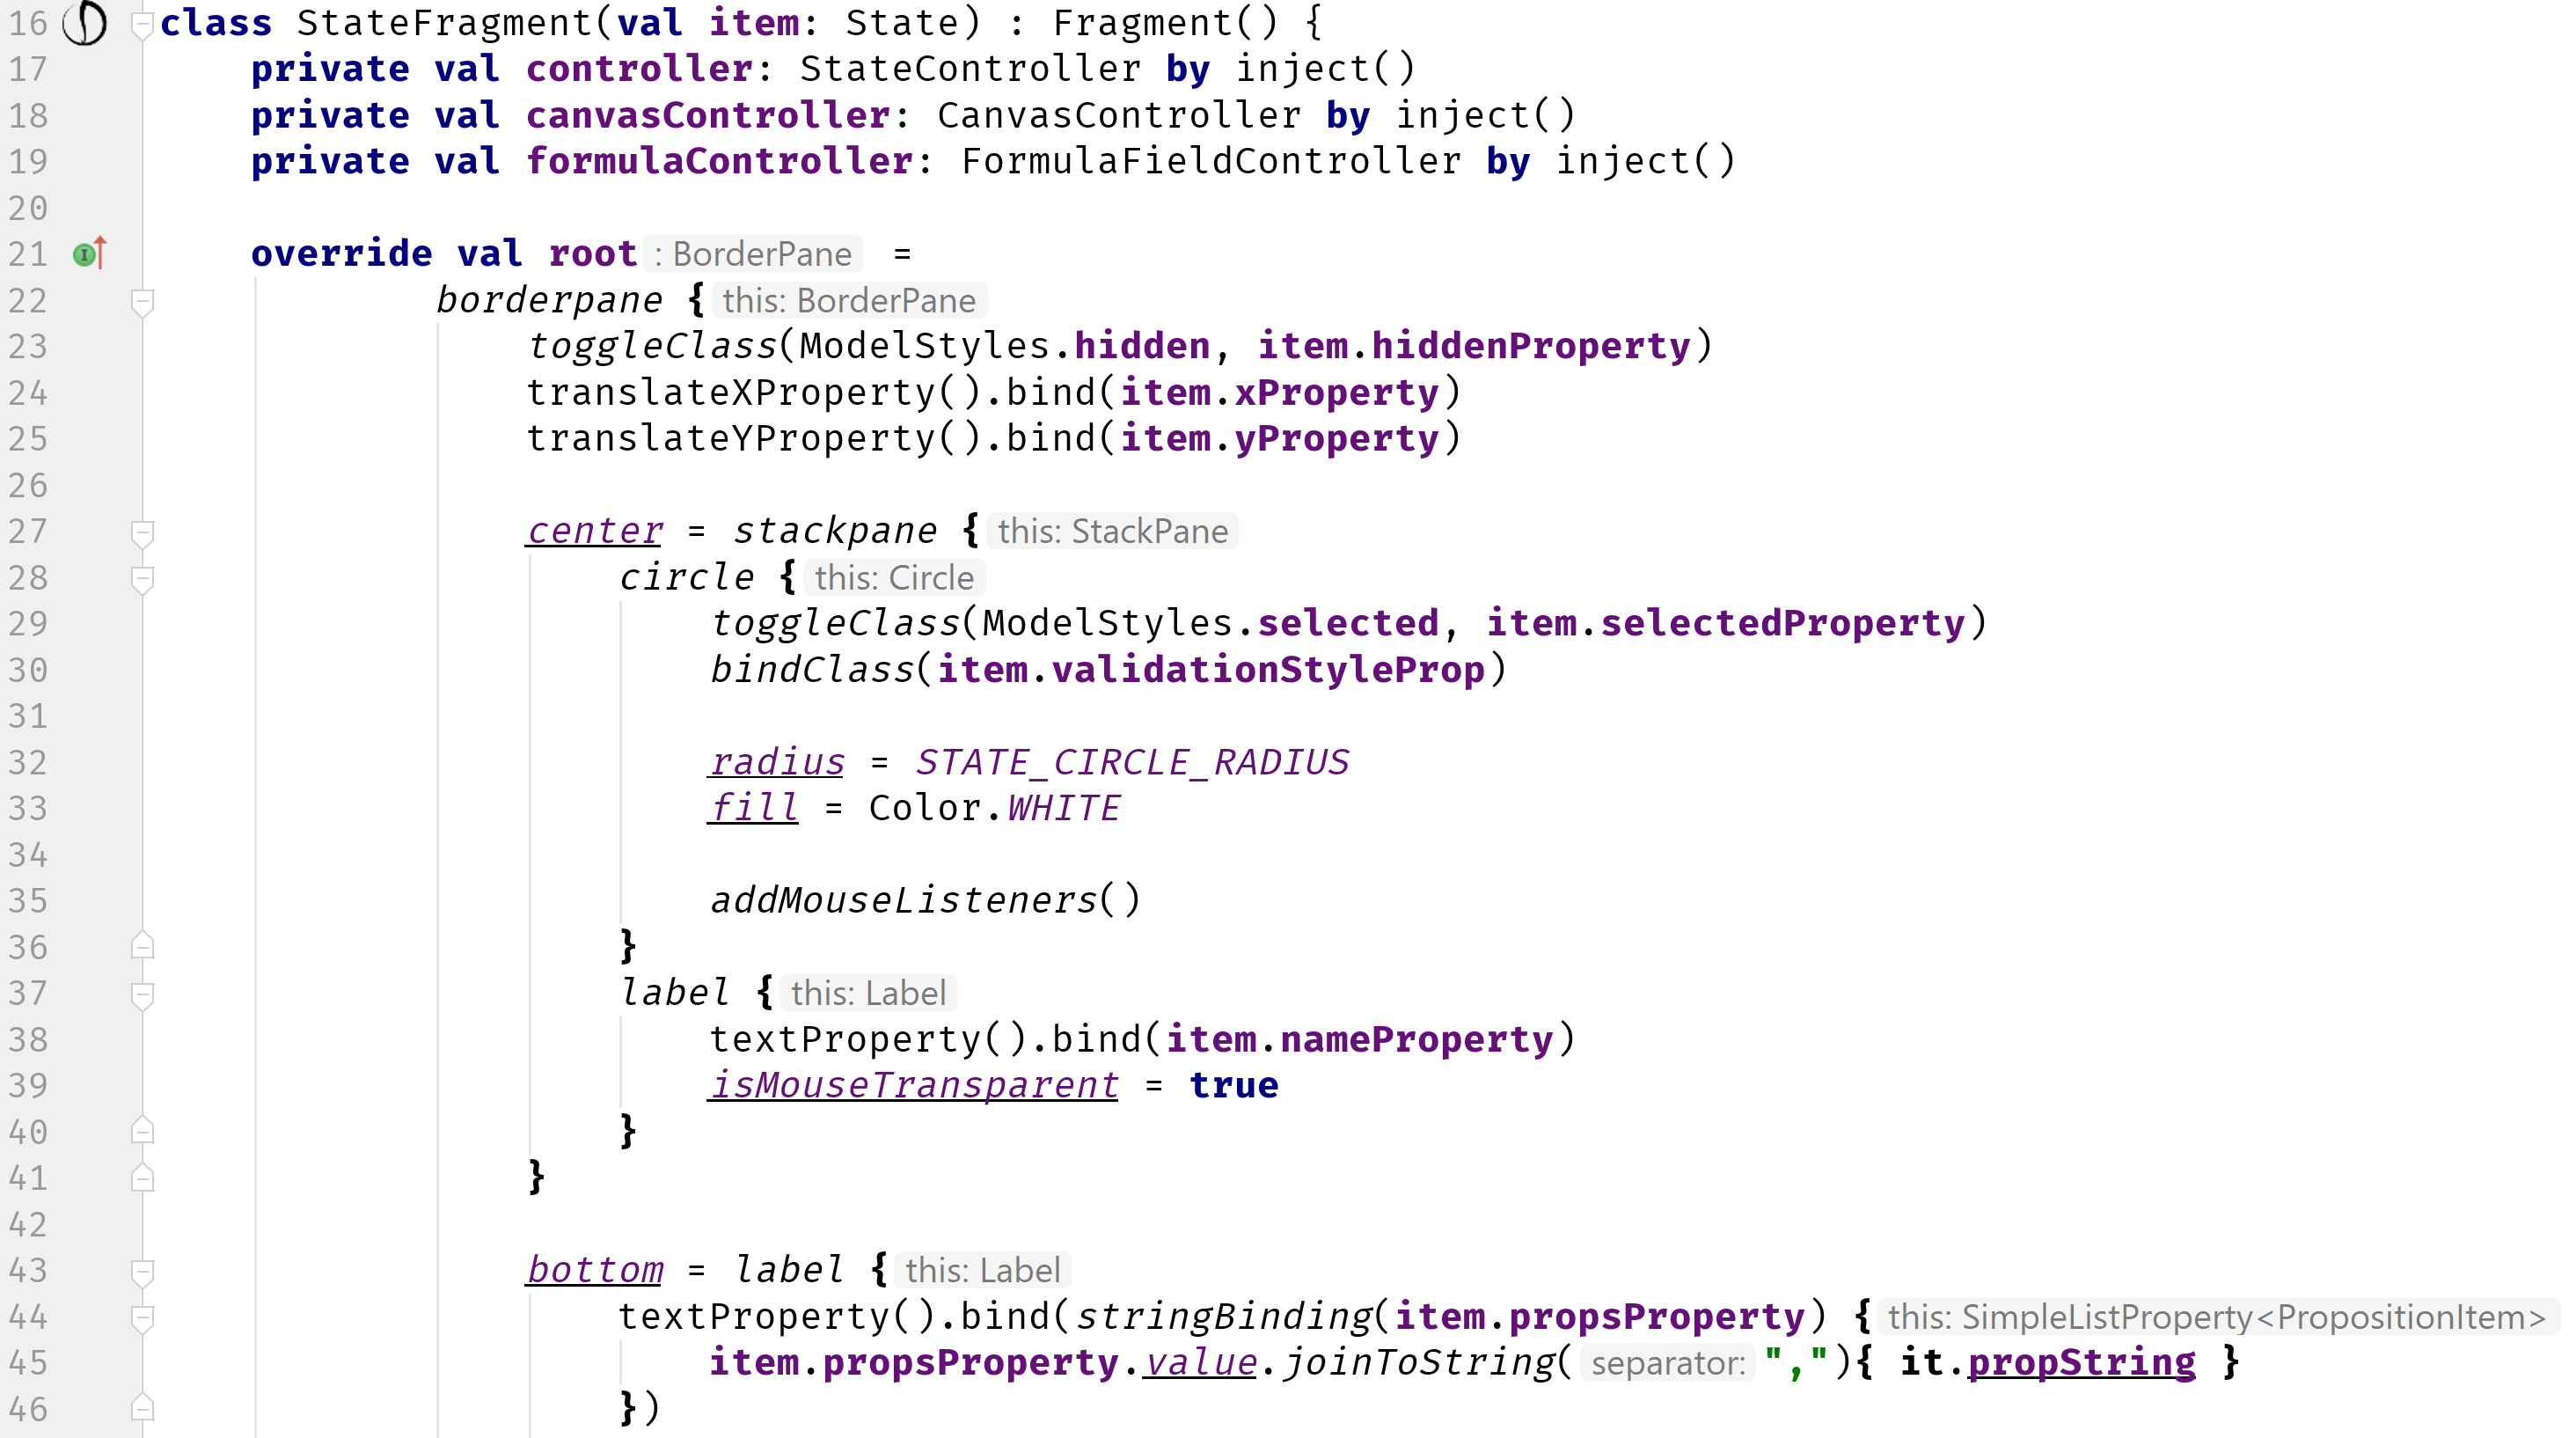
\includegraphics[width=\textwidth]{StateFragmentSnippet.png}
	\caption{Code handling how the UI components representing states are built. Note the conciseness due to implicit contexts.}
	\label{fig:StatFragSnip}
\end{figure}

For these reasons, we chose to implement our model checker in Kotlin, as prior to this project, most of my programming experience came from Java and its many libraries and as such, moving to a language with a far more concise syntax but still being able to lean on my previous experience was an excellent opportunity to learn something new. Going back to Java's wealth of libraries, the choice of GUI library to construct our user interface in fell on the \textit{de facto} standard Java GUI library, JavaFX, or more precisely; a Kotlin wrapper for it called TornadoFX \footnote{Library homepage at: \url{https://tornadofx.io}}. Our reasons behind choosing TornadoFX is that while JavaFX is a widely used and mature library with powerful features, we also feel its usage tends to produce somewhat clunky and verbose code. JavaFX does admittedly provide a solution to this; dumping most of the layout, styling and positioning of components into specialized XML-files. While this helps clean up classes representing UI-components however, it also makes dynamic component generation clumsier and tends to abstract away the component hierarchy in ways that makes it harder to reason around its structure. TornadoFX on the other hand, being a Kotlin library is able to present a much cleaner API by utilizing Kotlin features such as lambda expressions attached to receivers in order to create composable builder functions which generate your JavaFX component hierarchy in an imperative fashion. Additionally, the wrapper also has excellent and concise shorthands for creating dynamic bindings between UI components and observable sets of data, which we ended up using all throughout the application. However, I would say our biggest reason for choosing TornadoFX is probably how its composable builder functions allow you to circumvent the normally inverse order of declaration and creation of UI components compared to their order in the component hierarchy, which can be seen in Figure \ref{fig:StatFragSnip}.

%Later mention usage of this Java interoperability through JavaFX and Java hook for ANTLR

\subsection{Language and interpretation}

Besides creating an understandable user interface another large challenge we needed to solve was how to convert the plain text the user types in into data structures representing formulas to check. For this, we used a tool called ANTLR (ANother Tool for Language Recognition)\footnote{\url{http://www.antlr.org/}}. ANTLR is a powerful parser generator which based off of a set of grammatical rules, can be used to generate parsers which implement these rules. These grammatical rules can be broadly split into parser and lexer rules. Lexer rules are the low-level rules which define how the tool should convert individual characters or short strings of characters into lexical tokens which are then used by the more high-level parser rules to define how ANTLR should assemble these tokens together again. For a more concrete example, we have the entirety of \cname{}'s grammatical rules pictured in Figure \ref{fig:grammar}. Here we can see how this simple set of lexical rules handle converting symbols into tokens representing the various operators in our language, but also how our set of parser rules define all legal ways of combining these symbols into formulas. 
\begin{figure}[h]
	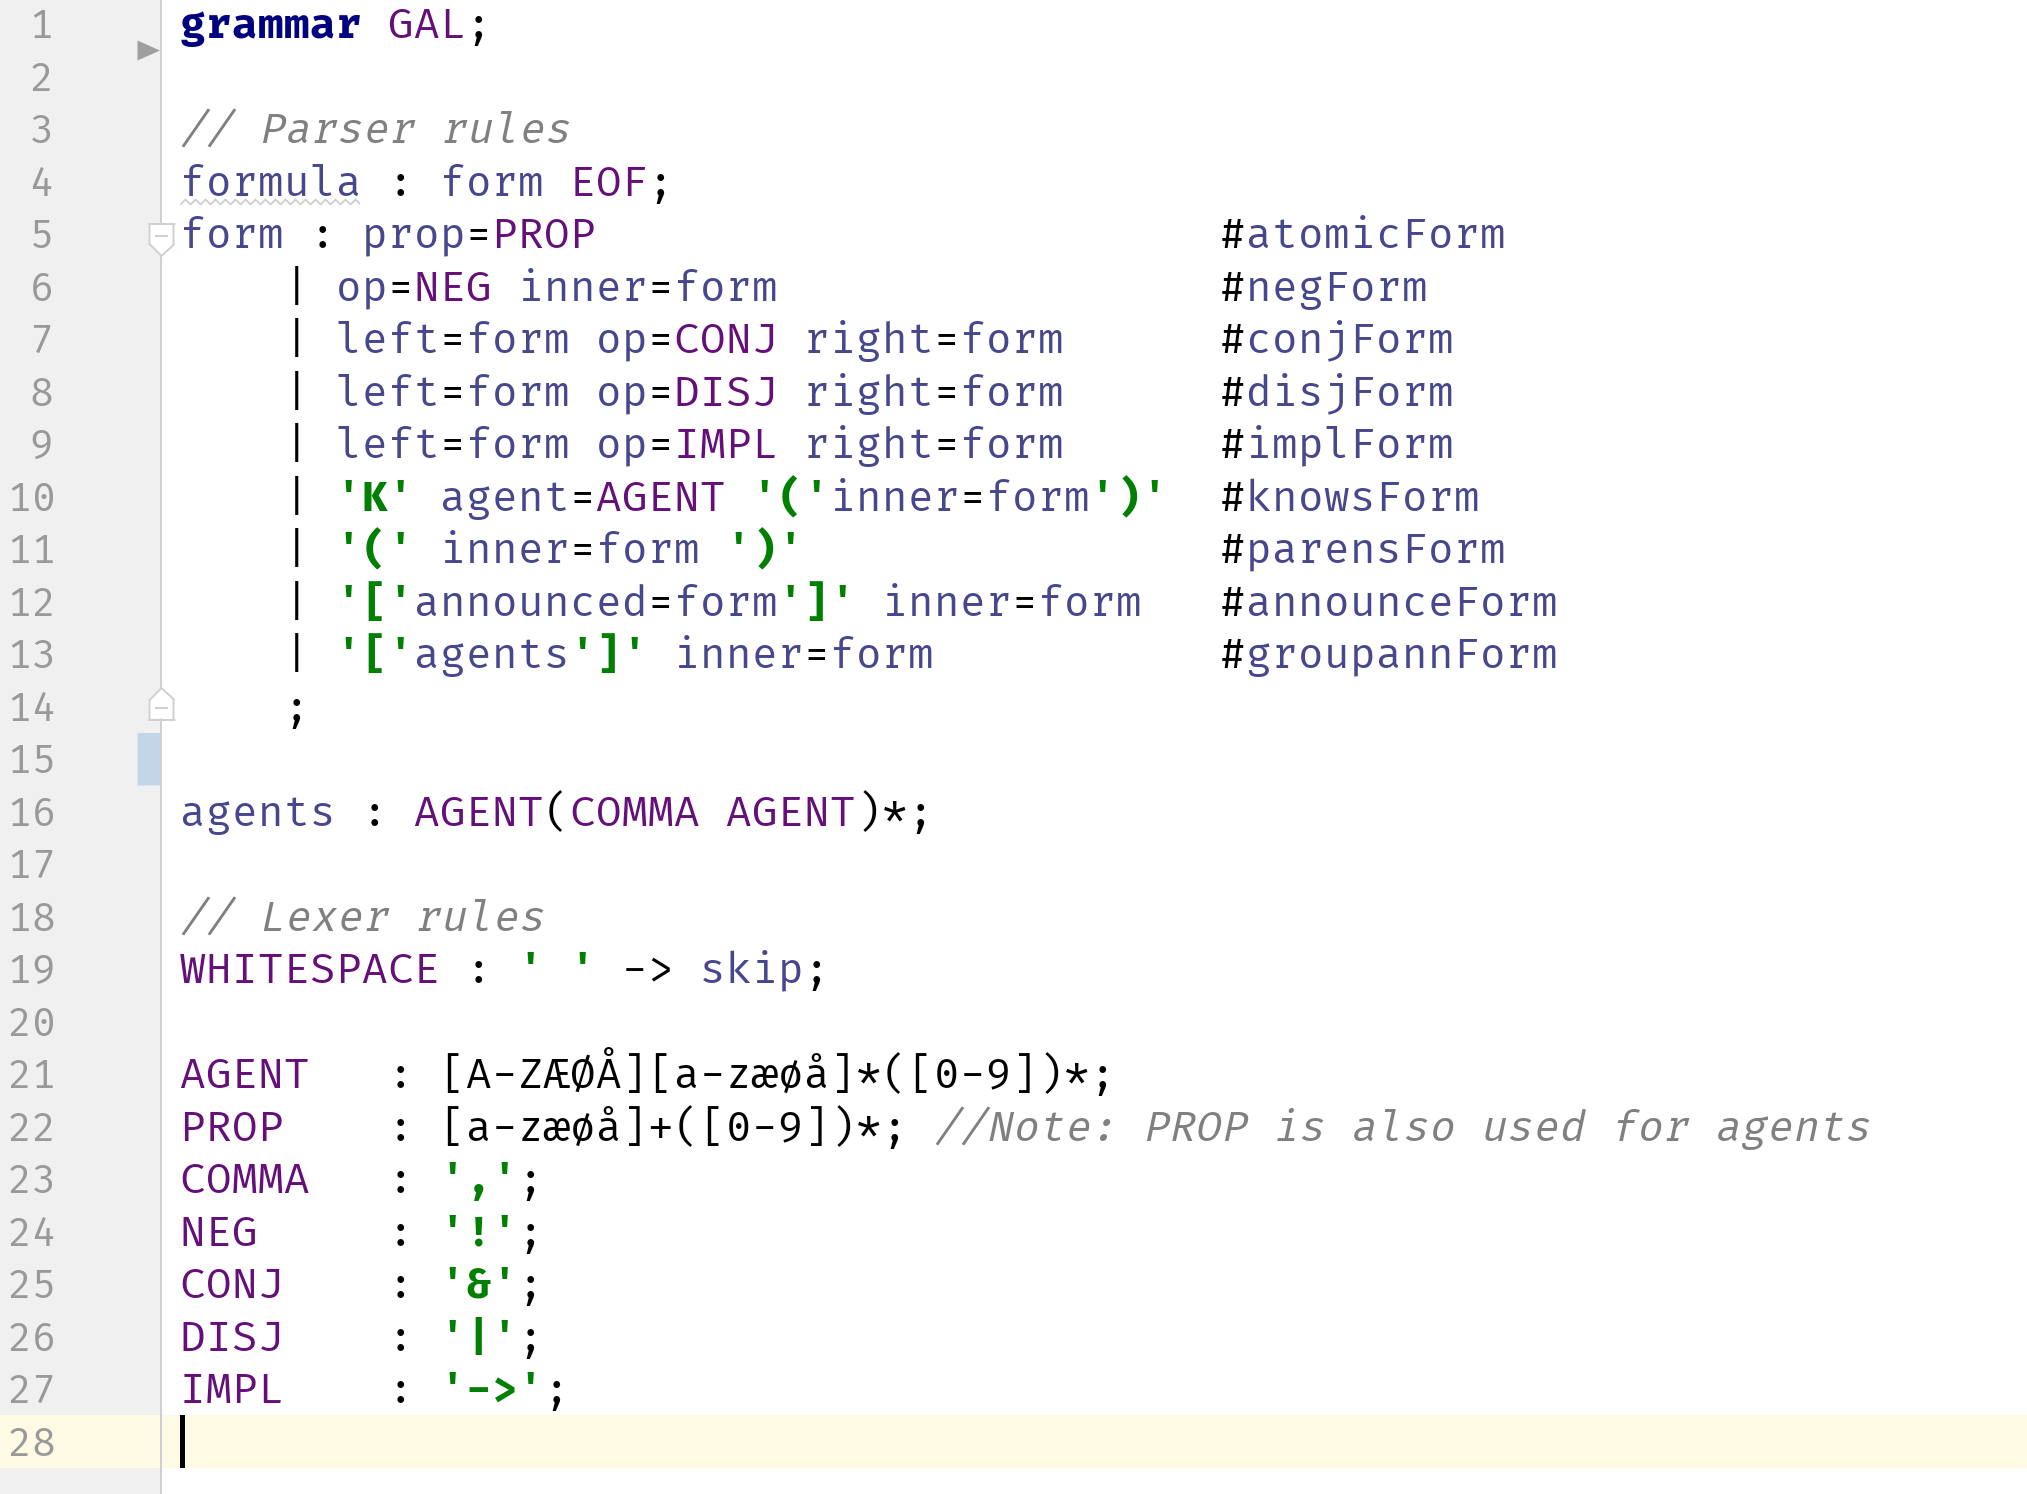
\includegraphics[width = \textwidth]{GALGrammar.png}
	\caption{Grammatical rules for parsing formulas in \cname with ANTLR.}
	\label{fig:grammar}
\end{figure}

For comparison, the language described by this ANTLR grammar can also be expressed as the following BNF (terminal symbols are underlined):

\begin{align*}
  \phi ~~&::=~~ \pi ~\big|~ \underline{!} \, \phi ~\big|~ \phi \, \underline{\&} \, \phi ~\big|~ \phi \,\underline{ | }\, \phi ~\big|~ \phi \, \underline{\text{-}\!>} \, \phi ~\big|~ \underline{K}\, \alpha\, \underline{(}\,\phi\,\underline{)} ~\big|~ \underline{(}\, \phi \,\underline{)} ~\big|~ \underline{[} \, \phi \, \underline{]} \, \phi ~\big|~ \underline{[} \, C \, \underline{]}\, \phi\\
  C ~~&::=~~ \alpha ~\big|~ \alpha \, \underline{,}\, C
\end{align*}

where $\pi$ (propositions) and $\alpha$ (agents) are sets of terminal symbols characterized as follows:
$\pi$ contains all strings of at least one lower case letter and possibly followed by a string of digits, matching the following regular expression:
$$
[\text{a-zæøå}]^+[0-9]^*
$$
$\alpha$ is a single upper case letter followed by a (possibly empty) string of lower case letters, and subsequently a (possibly empty) string of digits, as described by the following regular expression:
$$
[\text{A-ZÆØÅ}][\text{a-zæøå}]^*[0-9]^*
$$

One thing to note in Figure \ref{fig:grammar} are the symbols used to represent negation, conjunction and disjunction. As previously mentioned, since the commonly used symbols for these operators do not exist on normal keyboards, the UI would either need extra buttons to facilitate inserting these symbols or use more easily accessible surrogate symbols. Another small concession I had to make in order to differentiate between agents and propositions, was to require that agent names be capitalized, as I would otherwise have to resort to using different symbols to differentiate between regular public announcements and group announcements. 

\begin{figure}[h]
	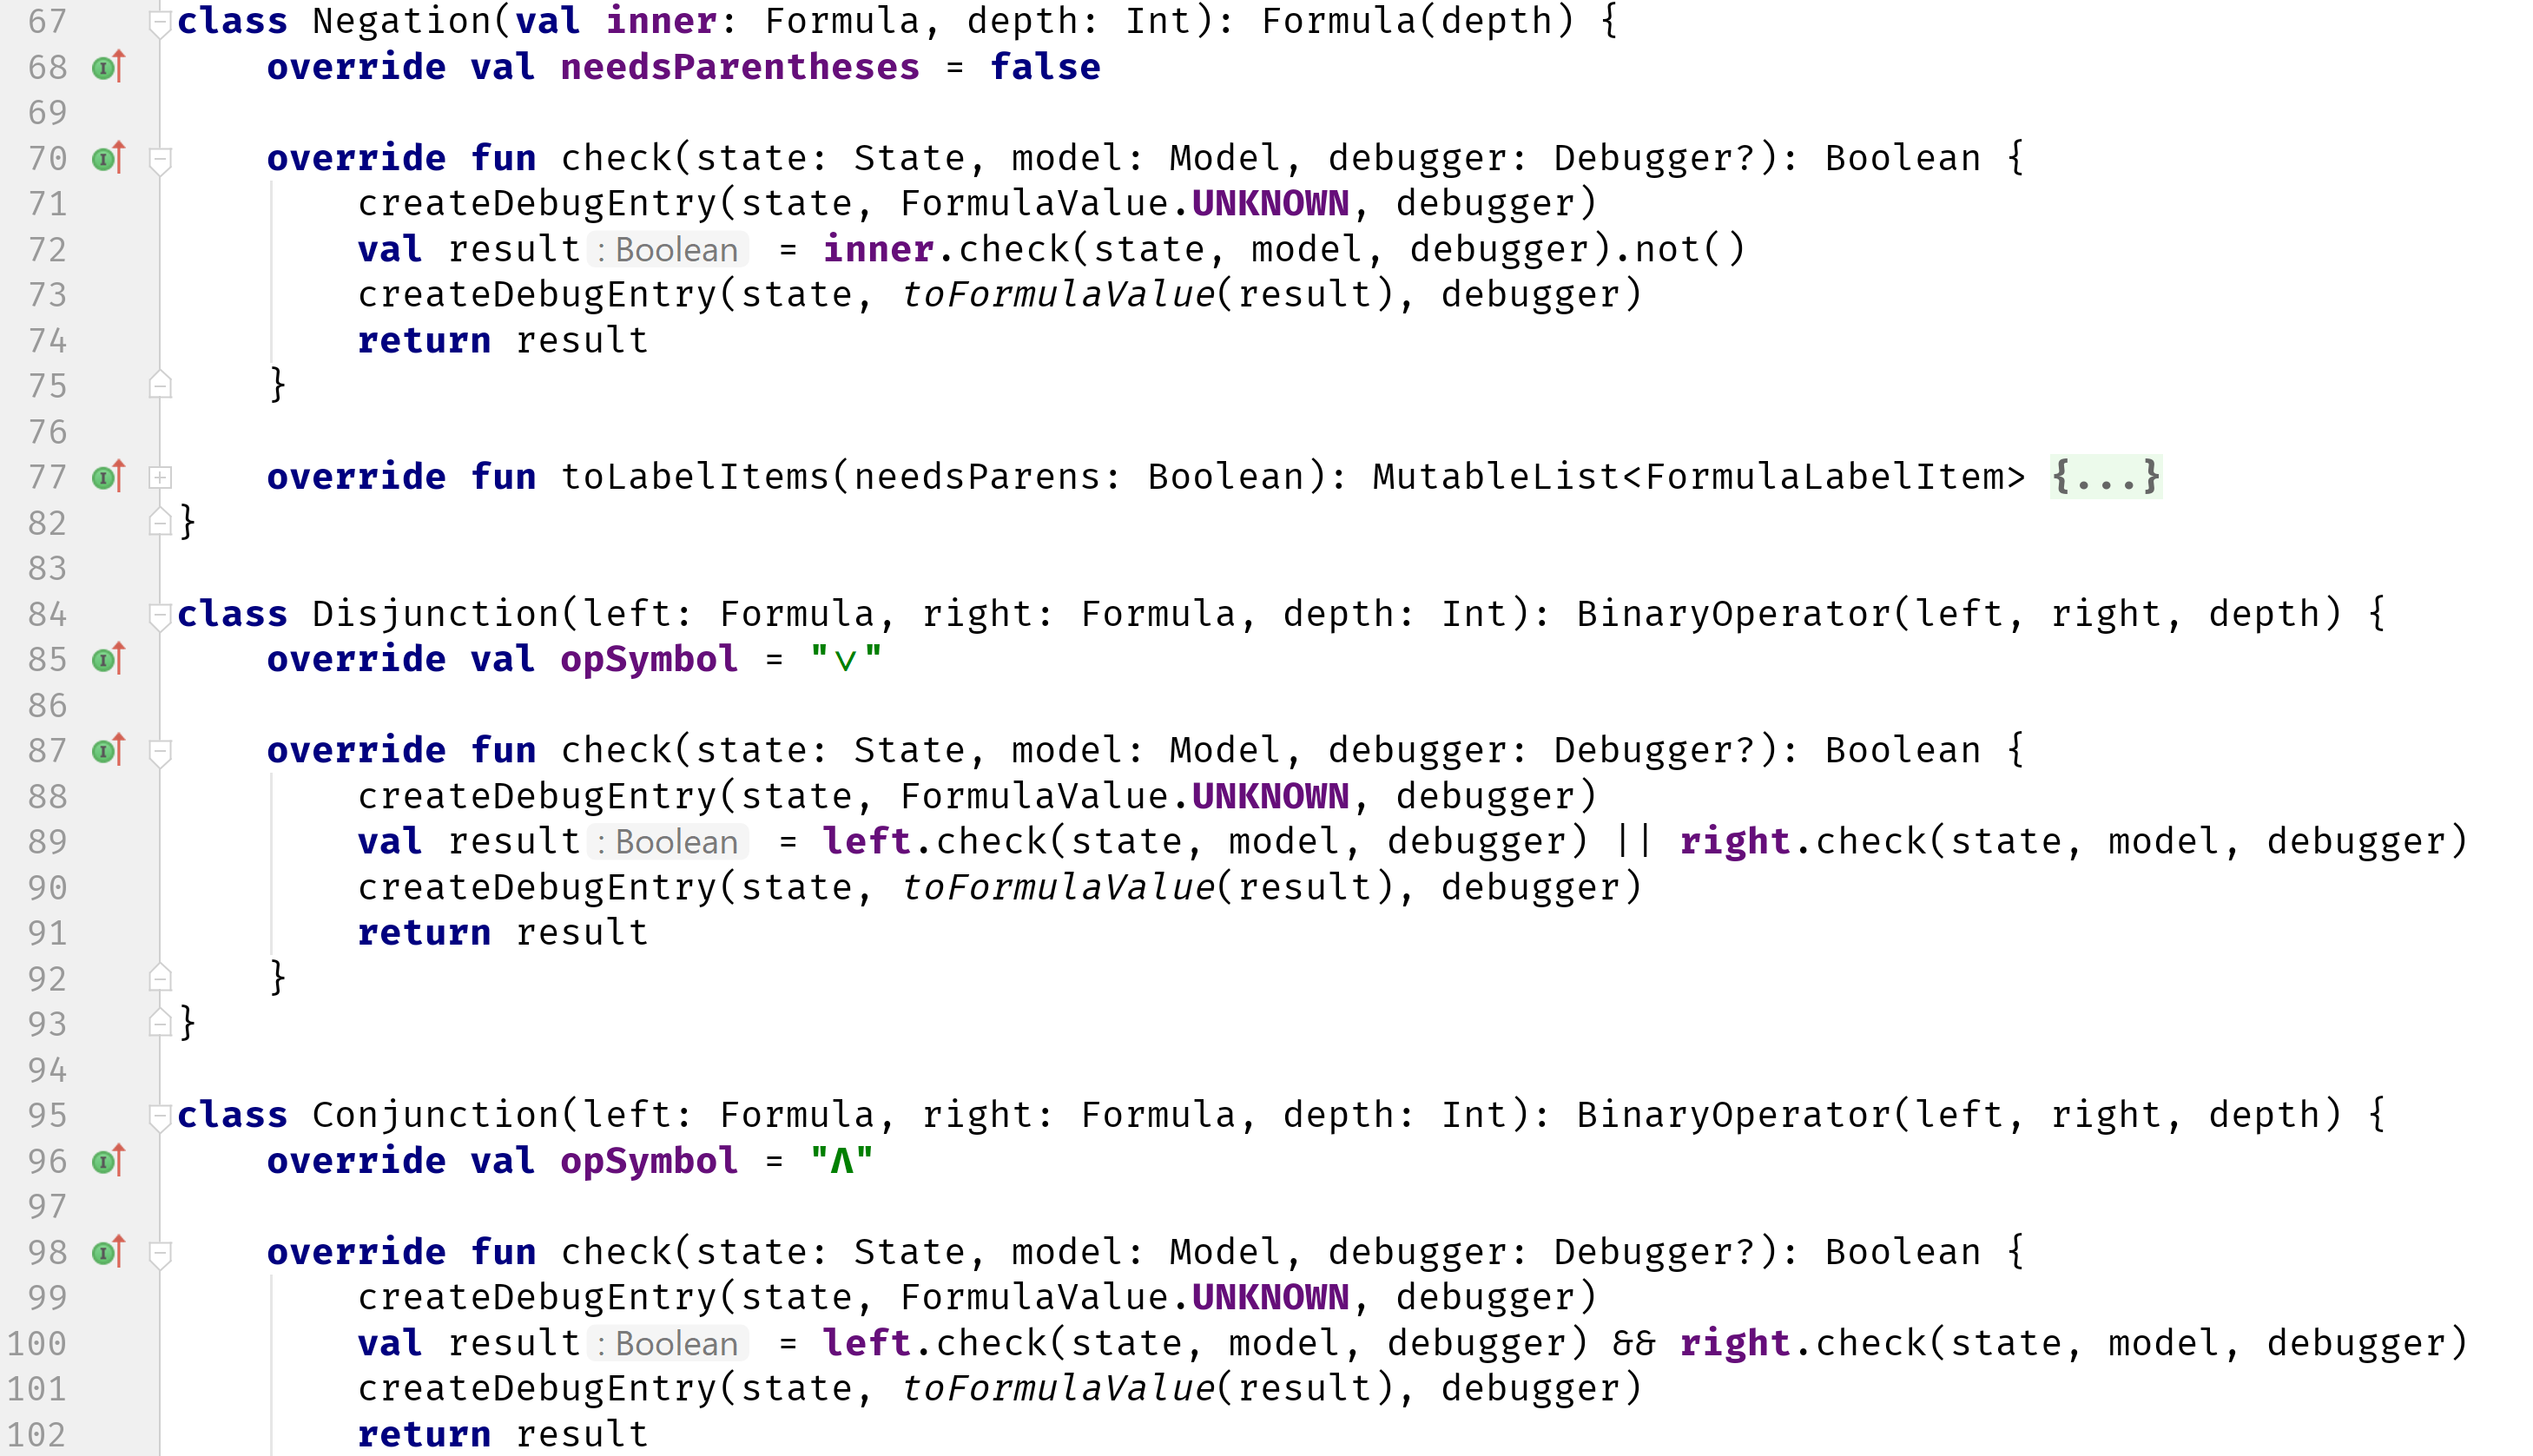
\includegraphics[width=\textwidth]{FormulaImpl.png}
	\caption{Snippet showing how various operators are implemented}
	\label{fig:formulaImpl}
\end{figure}

The parser that ANTLR generates from this simple grammar is then used to convert the user's plain text input into instances of our Kotlin classes which represent the various operators in our language. An interesting thing to note here however is that not only does it create instances of our operators, but it also instantiates them in order of traversal as it builds the formula tree, conserving the structure of this tree as it is rebuilt using our Kotlin-implementations of the operators. One of the more elegant aspects of our design is how these operators were implemented; with each operator extending an abstract formula class and simply overriding it's `check'-function with their own semantics, as can be seen in Figure \ref{fig:formulaImpl}. Also note how the constructors of each operator also takes other formulas as their parameters, allowing us to directly implement the BNF definition of GAL presented earlier through constructor typing alone.

\subsection{Kripke structures and UI components}

As the focus when making the application was mainly on making it as easy to use as possible while presenting information in a visual manner that is easy to grasp, we ended up making several deviations from the more commonly seen logical definitions of epistemic models. In Definition \ref{def:model} we present $\rels$ as a function from each agent to their respective equivalence relation for every state in the model. In \cname{} however, we instead chose to represent these equivalence relations as a set of edges represented as objects consisting of a pair of states and the set of agents that consider this pair of states indistinguishable. The reasons for this ties back into how we wanted to present an interactive view of the models in our application, as TornadoFX, our GUI library makes it far easier to represent each component of our models as concrete objects, which we can then bind UI-components to. Since each edge also has a reference to the set of agents it is valid for, this makes it trivial for us to visualize this information as well. 

Building on these changes, we additionally made each state aware of which edges it is connected to, trivializing the logic behind finding indistinguishable states for a given agent, as we simply filter the set of edges our state is connected to based on which edges are relevant for our given agent and return the list of states these edges lead to. While these are deviations from how Kripke structures are more commonly defined, we argue that they make for a much cleaner programmatic representation as they allowed us to simplify both visualization as well as our implementation of the semantics.

We also chose to flip the valuation function by letting states hold a reference to a set of propositions which are satisfied in them, rather than each proposition being linked to the set of states they are satisfied in. Our reasoning here is much the same as for changing how we handle indistinguishability; it allowed us to simplify how we present which propositions are true in each state. We do so by applying a mapping function to these sets of propositions to generate labels in our UI which can then be automatically updated whenever this underlying set of propositions updates. This is far simpler than having to go through the entire set of propositions each time the user updates which propositions a given state satisfies. The code responsible for binding this set of propositions to labels can be seen at the bottom of Figure \ref{fig:StatFragSnip}.


\subsection{Model checking}

Going back to our presentation of \cname{} in the previous chapter, we described that the tool provides two main modes of checking formulas, which we will now discuss the implementation of. The first and simplest of these modes is simply checking which of the states in the user's model satisfy the input formula. With our implementation of formulas, we can simply do this by invoking the formula's check-function on each state in our model, styling the state-component based on the outcome of this checking, as can be seen in Figure \ref{fig:CheckingFunction}. We also previously described how \cname{} allows its user to mouse over the various subformulas in order to check how they affect the valuation of their containing formula. We implemented this by tying each symbol in the displayed formula to the subformula it represents and then calling the same check-formula with this subformula.

\begin{figure}[h]
	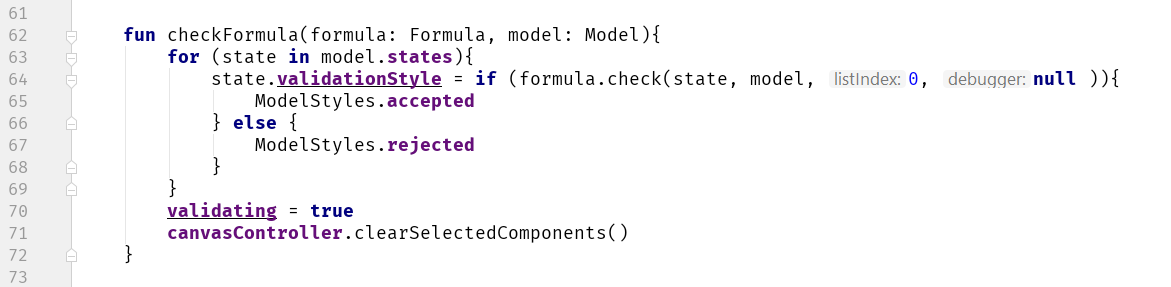
\includegraphics[width=\textwidth]{CheckingFunction.png}
	\caption{Function responsible for highlighting which states in our model satisfy the input formula}
	\label{fig:CheckingFunction}
\end{figure}

How step-by-step visualization works is somewhat more involved. A high-level description of how it is implemented is that the `debugger' hooks into the $check$ function of the formula, and logs each step of the checking process. Looking back at Figure \ref{fig:formulaImpl}, this can be seen through our calls to \textit{createDebugEntry}, which is responsible for logging the valuation of each operator in the user's formula before and after every call to this $check$ function.

Each log then carries information about what the valuations of each operator was at that point in the process, so that this checking process can be played back and visualized in the form of showing the various operators change color as their valuations become known. 

Briefly touching upon saving and loading of models as mentioned at the end of the last chapter, as our models are plain Kotlin (and by extension Java, as Kotlin is fully interoperable with Java) objects, reading and writing them to files is simply a matter of using the built-in tools in the Java library to serialize them and write them to file, as seen in Figure \ref{fig:serialization}. While using the JVM library for writing and reading models from files saved us a lot of time, it does however also mean that the models are written in a plain binary format. While it would have been nice to store our models in a more widely-used format so that more complex models could be visualized and edited in more powerful graph editing tools such as Gephi\footnote{https://gephi.org/}, this was left as future work since I estimated it would take too long to implement compared to the value it would provide.

\begin{figure}
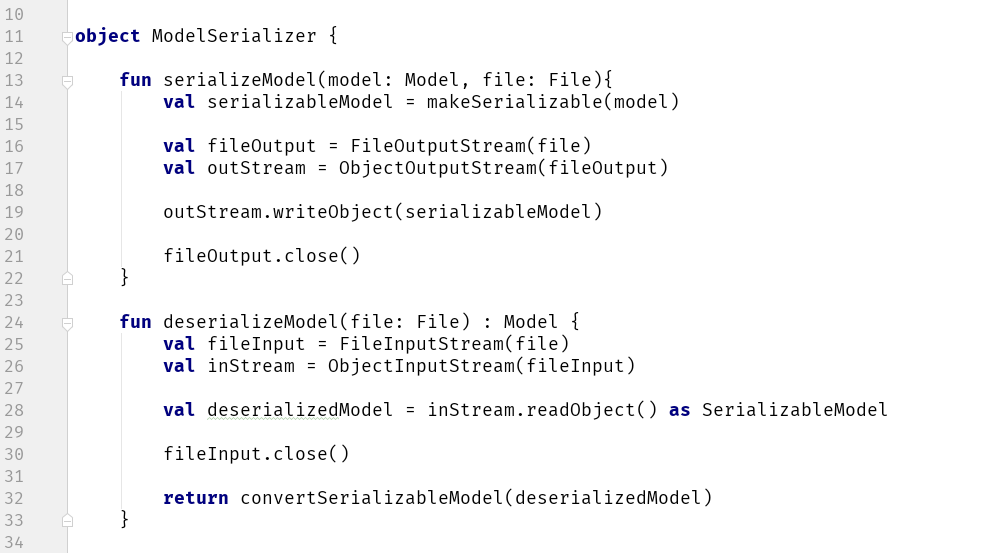
\includegraphics[width=\textwidth]{SerializationCode.png}
\caption{Code behind reading and writing models to file}
\label{fig:serialization}
\end{figure}

%Features - should explain how each of these are implemented \\\\


%Saving and loading models, as well as importing other models into the current model (Useful for importing commonly used components)\\


%Compare with implementations in DEMO, advantages/disadvantages of wrapping things in objects ect.\\
%We use observable objects with pointers to each other, DEMO simply has arrays of integers, which are more lightweight and potentially easier to manipulate, but much harder to render \\
%Discuss differences with logical definitions\\
%Provide walkthrough of how program checks formulas\\

%Debugger, DebugLabels, attaching itself to checking process of formulas, lots of shady voodoo to link DebugEntries in sidepanel to DebugLabels next to each state in order to update them as the user navigates through entries\\

%Debugger inserts callback into CanvasController to know when the user selects a state\\
%List of checking steps has onChange() callback telling the Debugger to apply the valuation map for that step to all formula labels\\

%Checking: Everything up to knowledge is roughly equivalent to logical definitions, minus flipped valuation function. Knowledge is similar, but instead of having an equivalence relation for each agent, each state is instead connected to other states through a set of edges which hold for a set of agents. If 


%Checking, recursive, 'logger' used to display process step-by-step\\

